\begin{figure*}[t]
  \centering
  \begin{tabular}{ccc}
    \hspace{-10mm}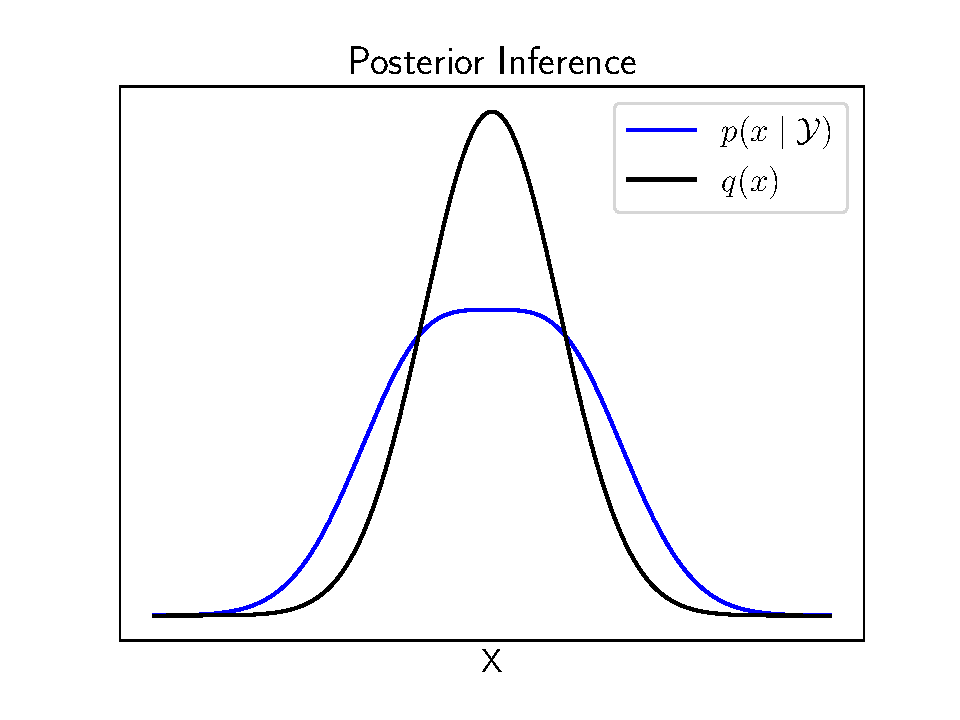
\includegraphics[width=0.37\textwidth]{inf_approx} &
    \hspace{-10mm}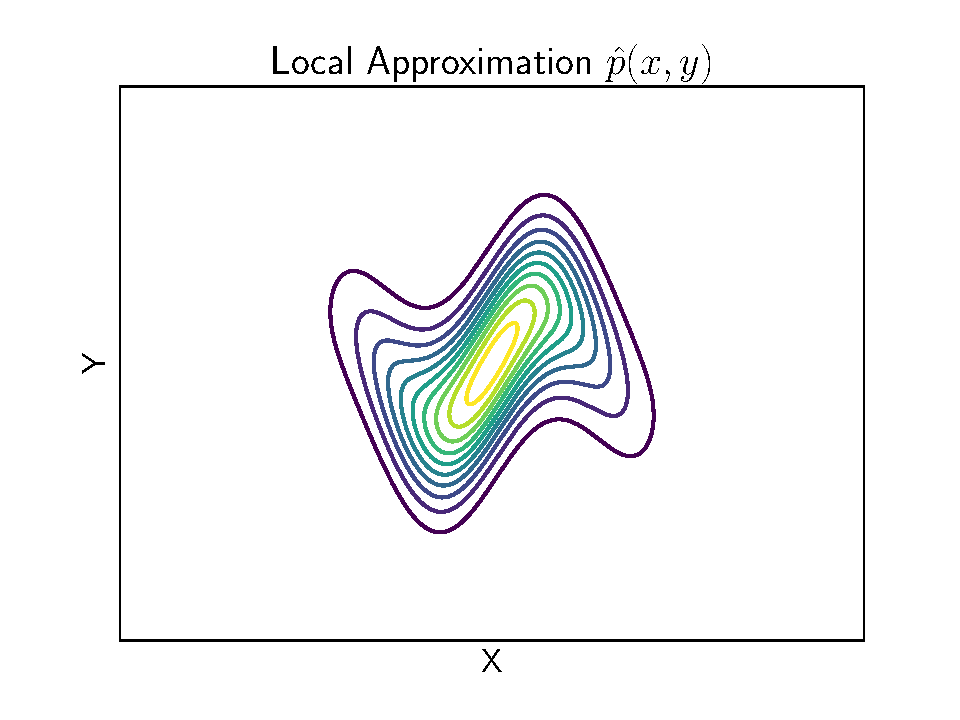
\includegraphics[width=0.37\textwidth]{augmented_dist} &
    \hspace{-10mm}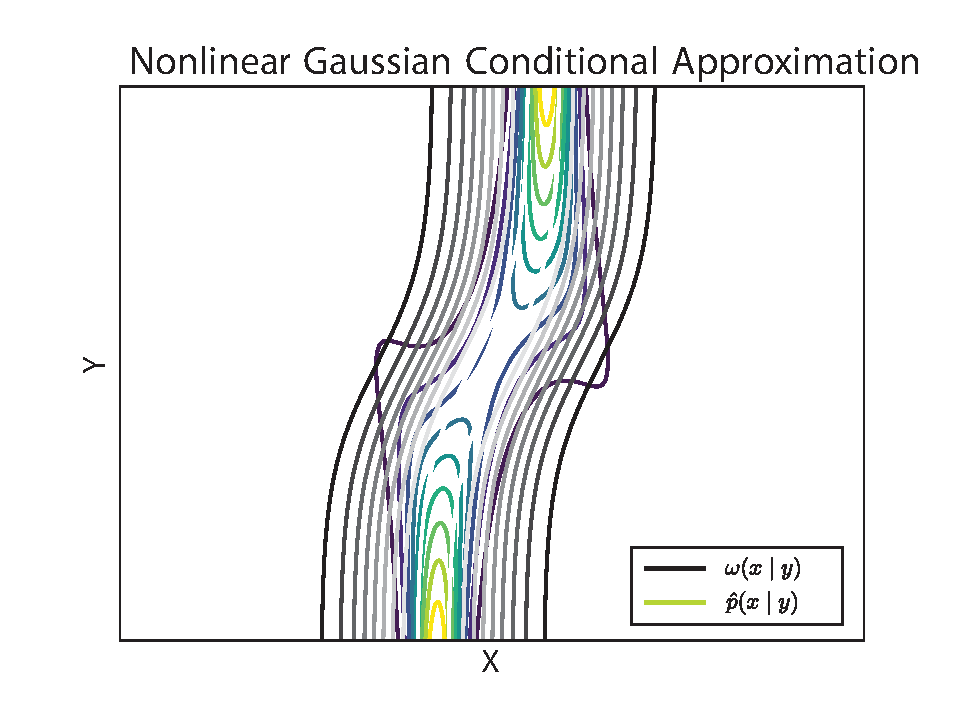
\includegraphics[width=0.37\textwidth]{nonlinear_approx}
  \end{tabular}

  \caption{\small \textbf{Variational information planning steps.}
    \emph{Left:} Given observations $\Ycal$ the posterior is
    approximated with a tractable family $q(x) \approx p(x\mid
    \Ycal)$.  \emph{Center:} To consider a new observation $y$, a
    local approximation is formed $\hat{p}(x,y) = q(x) p(y \mid x)$
    using the forward model.  \emph{Right:} The auxiliary distribution
    $\omega(x\mid y)$ minimizes $\KL{\hat{p}(x\mid y)}{\omega(x\mid
      y)}$ to bound $I(X;Y)$.  When the auxiliary distribution is in
    the exponential family we achieve efficient updates, yet allow
    nonlinear dependence on the conditioning variable $y$, thus
    yielding tighter MI bounds.}

  \label{fig:approx}
\end{figure*}

Motivated by the challenges of sample-based MI estimation, we
introduce an efficient variational approach.  Beginning with a lower
bound on MI, we extend this to sequential decision making and
formulate the calculations for a model where observations are
conditionally independent.  Finally, we show how VIP can be applied to
a more complex model common in the related setting of active learning.

\subsection{Variational Information Bound}
For any valid conditional distribution ${\omega(x\mid y)}$, Gibbs' inequality
admits the following lower bound on MI:
\begin{equation}\label{eq:varmi}
  I(X;Y) \geq H(X) + \EE_p[ \log \omega(X\mid Y) ].
\end{equation}
This bound has been independently explored in various
contexts~\citep{agakov2004algorithm, mohamed2015variational,
  gao2016variational, chen2018learning}.  In the remainder of this
paper we refer to ${\omega(x\mid y)}$ as the \emph{auxiliary
  distribution}.  The dual planning problem maximizes the
bound~\eqref{eq:varmi} w.r.t. this auxiliary distribution.  Each stage
of planning requires the posterior mutual information, ${I(X,Y_t\mid
  \Dcal_{t-1})}$ bounded by,
\begin{equation}
  H(X\mid \Dcal_{t-1}) + \EE_p[ \log \omega(X\mid Y) \mid
    \Dcal_{t-1}].
  \label{eq:varmi_seq}
\end{equation}
Calculating \EQN\ref{eq:varmi_seq} involves expectations over the
posterior distribution ${p(x,y_t \mid \Dcal_{t-1})}$, thus efficient
sequential planning requires further approximations.  The procedure is
most easily understood for a simple model of conditionally independent
observations, which we now discuss before moving to more complicated
settings.

%% First, variational inference yields the posterior approximation
%% \mbox{$q(x)\approx p(x\mid \Dcal_{t-1})$}.  Then, we construct a local
%% approximation over the joint distribution for each hypothesized
%% action,
%% \begin{equation}
%%   \hat{p}_a(x,y_t) \approx p_a(x,y_t\mid \Dcal_{t-1})\quad \text{For}\;
%%   a=1,\ldots,A.
%%   \label{eq:local_approx}
%% \end{equation}
%% Finally, we perform planning by optimizing a lower bound with respect
%% to an auxiliary distribution \mbox{$\omega(x\mid y_t)$} and select the
%% maximizing action $a_t$ for the next time step.  See
%% \FIG\ref{fig:approx} for an illustration.  

\subsection{Conditionally Independent Observations}

Consider the model in \EQN\eqref{eq:conditional_indep_joint} where
observations $y_1,\ldots,y_t$ are independent, conditioned on $x$.
Given the variational approximation \mbox{$q(x) \approx p(x \mid
  \Dcal_{t-1})$} we form a local approximation of the distribution
over the future measurement at time $t$,
\begin{equation}\label{eq:local_approx}
  \hat{p}_{a}(x,y_t) \equiv q_{t-1}(x) p_{a}(y_t \mid x) \approx p_a(x,y_t\mid \Dcal_{t-1}).
\end{equation}
Here, $p_{a}(y_t \mid x)$ is the true likelihood under the
hypothesized action $a$.  We then bound the MI under
$\hat{p}(\cdot)$ as,
\begin{equation}\label{eq:varmi_approx}
  H_{\hat{p}}(X) + \max_{a, \,\omega}  \;\EE_{\hat{p}_a}\left[ \log \omega(X \mid Y_{t})
  \right].
\end{equation}
Under this model the marginal entropy $H(X)$ is constant during
planning and can be ignored.  The bound~\eqref{eq:varmi_approx} can be
evaluated in parallel for all actions $1,\ldots,A$.
\FIG\ref{fig:approx} illustrates the role of each approximation in a
single planning stage, and how the approximations relate to the target
distributions.  \EQN\eqref{eq:varmi_approx} bounds mutual information
under the local approximation $\hat{p}(\cdot)$.  The conditions
ensuring \EQN\eqref{eq:varmi_approx} is a reliable surrogate to
\EQN\eqref{eq:varmi_seq} are the same as those for variational
inference to be effective.

\subsection{Semi-Supervised Annotation Model}\label{sec:annotation}

We now consider a more complicated model consisting of semi-supervised
\emph{annotations} $\{y_n\}_{n=1}^N$, a fixed set of data $\{z_n\}_{n=1}^N$,
and latent quantities $x$.  The joint distribution is given by,
\[
  p(x,y,z) = p(x) \prod_{n=1}^N p(z_n, y_n \mid x).
\]
Variations of this model are common
in active learning contexts~\citep{settles2012active}.  For example,
$y_n$ may be a class label for data element $z_n$.  Each learning
stage selects the most informative annotation $y_{n^*}$ maximizing
posterior MI:
\begin{equation}
  n^{*} = \argmax_n I(X;Y_n \mid \Dcal_{t-1})
\end{equation}
%% Where $p(x,y_n \mid \Dcal_{t-1}) \propto $ \vspace*{-3mm}
%% \[
%%   p(x \mid \Dcal_{t-1} \setminus \{z_n\}) p(z_n \mid
%%     x ) p(y_n \mid z_n).\vspace*{-3mm}
%% \]
%% Here, $p(x \mid \Dcal_{t-1} \setminus \{z_n\})$ represents the
%% posterior distribution after removing $z_n$ from the data, which
%% intuitively avoids double counting data $z_n$.
%%
Here $\Dcal_{t-1}$ is the set of all data $z_1,\ldots,z_N$ and the
currently observed annotations.  To form a local approximation
$\hat{p}(\cdot)$ we assume a posterior approximation that is a product
of nonnegative normalizeable factors,
\begin{equation}
 q(x) \propto \prod_{n=1}^N \psi_n(x)
\end{equation}
In expectation propagation (EP) parlance, factors $\psi(x)$ can be
interpreted as messages in a factor graph.  Similarly, EP defines the
concept of a \emph{cavity distribution} $q^{\backslash n}(x) \propto
q(x) / \psi_n(x)$, which expresses the posterior approximation having
removed $z_n$.  Our local approximation is then analogous to the EP
\emph{augmented distribution},
\begin{equation}
  \hat{p}(x, y_n) \propto q^{\backslash n}(x) p(z_n, y_n \mid x).
\end{equation}
The MI lower bound is then identical to~\eqref{eq:varmi_approx}.  More
complicated models with nuisance variables that must be integrated out
for planning can be handled in a similar manner, with additional
marginalization.  We consider such a setting for the labeled LDA
active learning example in Sec.~\ref{sec:llda}.


